\documentclass[a4paper,12pt]{article}

\usepackage{anysize}
\marginsize{30mm}{20mm}{20mm}{20mm}
\usepackage[utf8]{inputenc}
\usepackage[english]{babel}
\usepackage[style=ieee,backend=biber]{biblatex}
\addbibresource{FinalReport.bib}
\usepackage{amsmath}
\usepackage{graphicx}
\graphicspath{ {./generatedImages/} }
\usepackage{svg}


%opening
\title{Linear Direct Current Electromagnetic Motor with Liquid Eutectic Gallium-Indium Alloy Coil}
\author{Jason Guan}
\date{27 September 2019}
\begin{document}

\maketitle
\begin{center}
	892594255\\
	Department of Engineering Science\\
	Supervised by Dr. Bryan Ruddy
\end{center}

\newpage

\begin{abstract}
Abstract placeholder
\end{abstract}

\newpage

\section*{Acknowledgements}
Paul Roberts 

Steve Oldman 

Greg  

Nick, Suroosh, Mahsa and Yahya 

And of course, Dr. Bryan Ruddy 

\newpage

\tableofcontents

\newpage

\section{Introduction}
Background\\

Soft robots important \\

Methods of locomotion all new, each with different advantages and drawbacks \\

Lack of traditional locomotion options \\

Liquid metal wired electromagnetic motors presents a possible solution \\

Transferral of existing robotics locomotion corpus to soft robots \\

Also presents a possible advantage re: cooling by circulating the wires \\

Question Statement \\

Is it feasible to build an electromagnetic motor using liquid metal for wiring that can also be cooled via circulating metal in the wiring? \\

Aims \\

Design, build and characterise an electromagnetic motor with liquid metal coils\\

\newpage

\section{Design, Manufacturing and Assembly}
\subsection{Mathematical Modelling}
\subsubsection{Motor Force}
\begin{equation} \label{eq:emmfdef}
\mathcal{F}=\mathcal{R} \Phi
\end{equation}

\begin{equation} \label{eq:flux1}
\Phi_0 = \int{B\ dA}
\end{equation}

Under the assumption B is uniform, equation \ref{eq:flux1} becomes
\begin{equation}
\Phi_0 = BA
\end{equation}

\begin{equation}\label{eq:emmf1}
\begin{split}
\mathcal{F} & = R_m \Phi_0\\
& = \frac{l_m}{A_m}B_r A_m\\
& = l_m B_r
\end{split}
\end{equation}
$A_m$ cancels out demonstrated in \ref{eq:emmf1}

\begin{equation}\label{eq:emmfreal}
\mathcal{F}=R_g\Phi
\end{equation}

\begin{equation}\label{eq:emmfsubbed}
\begin{split}
l_m B_r & = \frac{\ln{\frac{r_{out}}{r_{in}}}}{2\pi l_c}\Phi\\
\frac{2\pi l_m l_c B_r}{\ln{\frac{r_{out}}{r_{in}}}} & = \Phi\\
\end{split}
\end{equation}

\begin{equation}\label{eq:fluxdef}
\Phi = BA
\end{equation}

Subbing equation \ref{eq:fluxdef} into \ref{eq:emmfsubbed} gives
\begin{equation}\label{eq:fluxsubbed}
\frac{2\pi l_m l_c B_r}{\ln{\frac{r_{out}}{r_{in}}}} = B_active A_active
\end{equation}

\begin{equation}\label{eq:activearea}
A_active = 2\pi l_c (r_{core}-r_{wireout} + 2r_{wireout} \frac{(layer+1)layer}{2})
\end{equation}
$l_c$ cancels out

\begin{equation}\label{eq:fluxdensity}
B=\frac{l_m B_r}{\ln{\frac{r_{out}}{r_{in}}}(r_{core}-r{wireout}+r_{wireout}(layer+1)layer)}
\end{equation}

\begin{equation}\label{eq:fbil}
F=BIL_{active}
\end{equation}

\begin{equation}\label{eq:activel}
l_{active} = \frac{l_{in}=l_{2}}{}
\end{equation}

\subsubsection{Heat and Temperature}
\begin{figure}[h]
\centering
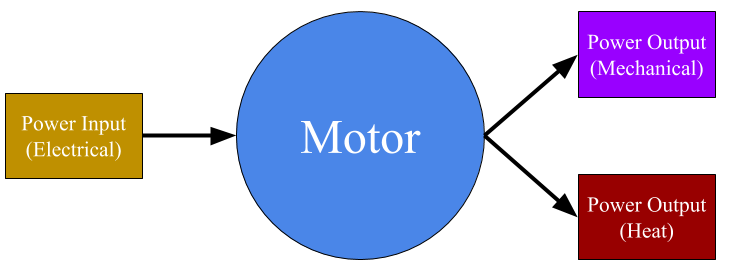
\includegraphics[scale=0.4]{motorheat.png}
\caption{Diagram of where motor heat comes from}
\end{figure}
something

\subsection{Optimisation Algorithm}
\begin{figure}[h]
	\centering
	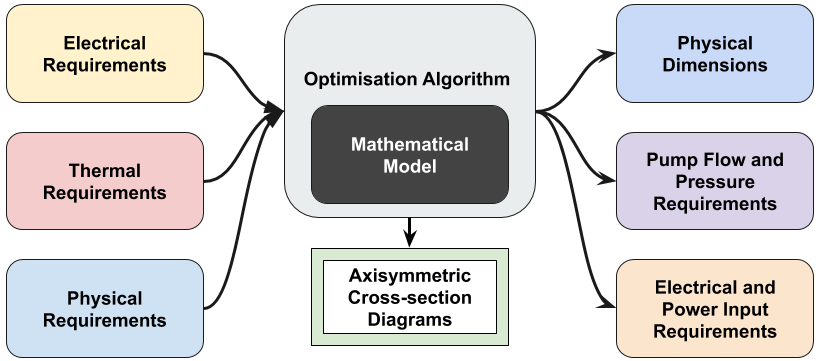
\includegraphics[scale=0.4]{optiAlgro.png}
	\caption{Diagrammatic representation of optimisaiton algorithm inputs and outputs}
\end{figure}
something else

\subsection{Physical Design and Manufacturing}
wires\\
magnet

\subsubsection{Shell}

\subsubsection{Core}

\subsubsection{Wire Bobbin}

\subsection{Assembly}

\subsubsection{Shell and Magnet Assembly}

\subsubsection{Wire Assembly}

\subsubsection{Health, Safety and Containment}

\newpage

\section{Experiment Designs and Results}

\subsection{Experiment 1: Force Characterisation}

\subsubsection{Method}

\subsubsection{Results}

\subsection{Experiment 2: Circulation Thermoregulation}

\subsubsection{Method}

\subsubsection{Results}

\newpage

\section{Discussion}

application to the original physical situation\\ 

comparison with related problems and other solutions\\

Critical assessment of significance\\

difficulty of the problem and how well it has been tackled\\

\cite{liuLiquidMetalMachine2016}

\newpage

\section{Conclusion}

\newpage

\section{Appendicies}

\newpage
References to previous works should be made in a consistent way. Specific references should be itemised in the Reference list, with any other more general material listed in a Bibliography. Only those books and papers actually consulted should be included. There are several variations on layout of reference lists; obtain advice from your supervisor and the library staff.  

\printbibliography
	
\end{document}
